\color{process}

\section{Konzeption}

In diesem Kapitel werden die Anforderungsdefinitionen des Projektes, mit Spezialisierung auf die verschiedenen Use Cases beschrieben.

\subsection{Anforderunsdefinitionen}

Um ein Schwarmverhalten für Kleinrobotern zu verwirklichen, indem verschiedene Komponenten miteinander interagieren, muss eine Basis geschaffen werden, damit der jeder Teilnehmer mit anderen kommunizieren kann. Die dabei teilnehmenden Komponenten sind in drei verschiedene Softwareanwendungen aufgeteilt.\\ 
Zum einen der Roboter, der Anfragen entgegennimmt und diese nach festgelegten Kriterien entsprechend verarbeitet. Dabei sendet jeder festgelegte Daten zur Synchronisation an eine höhere Instanz, die diese für eine Steuerung zur Verfügung stellt. Eine mobile App dient dabei zur Auswahl des Kontextes, in dem der Roboterschwarm gesteuert wird. Dazu erhält sie nach Start regelmäßige Daten zur Anzeige eines UI und sendet entsprechende Steuerungskommandos. Ein Desktopprogramm dient dabei als Backend und Kommunikationsschnittstelle, die die entschprechenden Anfragen weiterleitet und Daten zwischenspeichert, um diese anzuzeigen.\\
Dabei sind verschiedene Anforderungen für die Basissoftware von nöten:

\begin{itemize}
	\item Netzwerkanbindung
	\item Übergreifende Kommandostruktur
	\item Interpreter für Kommunikation
	\item User Interface
	\item Roboter Basisfunktionen
\end{itemize}

Zur Basissoftware werden zusätzliche Funktionen benötigt, die ein Schwarmverhalten zu erstellen. Um die verschiedenen Szenarien zu unterstützen wird einerseits ein Fahren des Roboters, sowie eine Positionsabhängiges Fahren, sowie ein definiertes Wendeprogramm in Abhängigkeit verschiedener Parameter wie Winkel und Zeit. Damit ist eine Zusammenarbeit der Roboter möglich zur Ausführung verschiedener Schwarmszenarien.

\newpage
\subsection{Softwarearchitektur}

Die Software besteht aus 3 Hauptkomponenten, dem Roboter, der Anfragen al JSON Objekte erhält und diese nach Kriterien entsprechend interpretiert und reagiert. Und nach dem Start eines Szenarios regelmäßige Daten an eine höhere Instanz sendet um die bestehenden Daten, wie Position auf den neuesten Stand zu bringen. 

\newpage
\begin{figure}[h]
	\centering
	\includegraphics[width=0.65\textwidth]{images/konzeption/Softwarearchitecture.png}
	\caption{Softwarearchitektur}
	\label{fig:softwarearchitecture}
\end{figure}

\newpage
\subsection{Steuerung}

\begin{figure}[h]
	\centering
	\includegraphics[width=0.65\textwidth]{images/Controling.png}
	\caption{Steuerung}
	\label{fig:steuerung}
\end{figure}

\subsection{Szenarien}

Zur Steuerung der verschiedenen Roboter wurden Szenarien entwickelt. Diese repräsentieren, in welchem Kontext die teilnehmenden Roboter gesteuert werden. Dabei gibt es verschiedene Unterschiede, von Anzahl der Roboter, Nutzer, sowie des Ziels des jeweiligen Szenario. Die Steuerung der Szenarien läuft dabei jeweils gleich ab, durch die im mobilen Gerät vorhandenen Gleichgewichtssensoren, werden Parameter zur Steuerung berechnet, die für die Ausrichtung und die Geschwindigkeit des entsprechenden Roboters zuständig ist.



% Verschiedene Modi

% Bild steuerung ??

\paragraph{Control}



\paragraph{Synchron}
\paragraph{Follow}
\paragraph{Flee}
\paragraph{Catch}

\subsection{Use Cases}
\subsubsection{Connect}

\begin{figure}[h]
	\begin{center}
		\includegraphics[width=0.8\textwidth]{images/use_cases/Connect.png}
	\end{center}
	\caption{Connect}
	\label{fig:UC_Connect}
\end{figure}

\noindent
Im Use Case Connect wird eine erste Verbindung durch die Eingabe der IP-Adresse zum Backend aufgebaut. Dabei sendet die Komponente, ob Roboter oder App eine Abbildung seiner selbst als Objekt dem Backend. Daraufhin startet das Backend die Verbindung indem es der Komponente entsprechende Verbindungskommandos zusendet. Sobald eine Reaktion in einer festgelegten Zeit erfolgt, akzeptiert das Backend die Verbindung und sendet die entsprechende Id für die Komponente. Ab diesem Moment ist die Komponente verbunden und ein Robot für Aktionen entsprechend verfügbar. Die Verbindungsinitialisierung dient hierbei der Verkürzung der Reaktionszeit, die bei einem Roboter sonst entsprechend hoch wäre.

\begin{figure}[!tbp]
	\centering
	\subfloat[Connect]{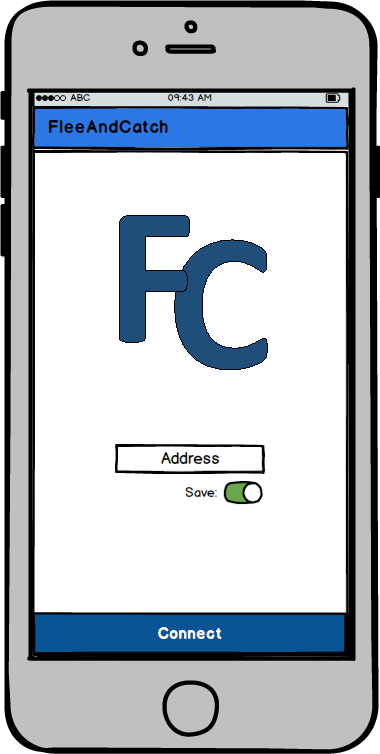
\includegraphics[width=0.4\textwidth]{images/mockups/Connection.png}\label{fig:Connect}}
	\hfill
	\subfloat[Home]{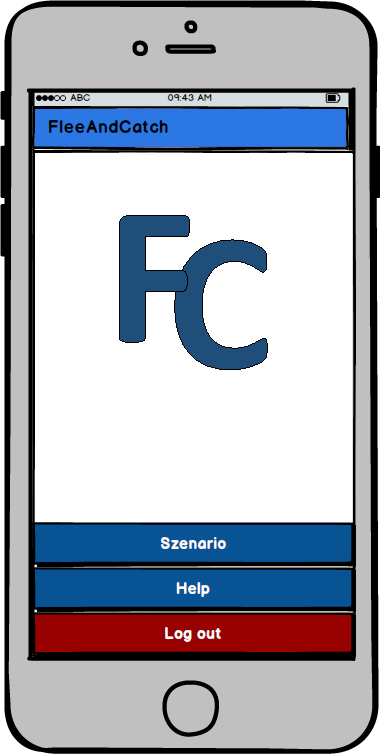
\includegraphics[width=0.4\textwidth]{images/mockups/Home.png}\label{fig:Home}}
	\caption{Connection}
\end{figure}

\subsubsection{Synchronization}

\begin{figure}[!tbp]
	\centering
	\subfloat[Update all]{\includegraphics[width=0.4\textwidth]{images/use_cases/Synchronization.png}\label{fig:UC_Synchronization}}
	\hfill
	\subfloat[Update]{\includegraphics[width=0.55\textwidth]{images/use_cases/Update.png}\label{fig:UC_Update}}
	\caption{Synchronization}
\end{figure}

\noindent
Im Use Case Synchronization werden Daten entsprechend des gesetzten Typen zwischen den Komponenten übertragen. Dabei können einerseits die Roboter als Objekte, oder ganze Szenarien übertragen werden. Dies dient zur Gegenseitigen Synchronisierung der Daten.

\begin{figure}[!tbp]
	\begin{center}
		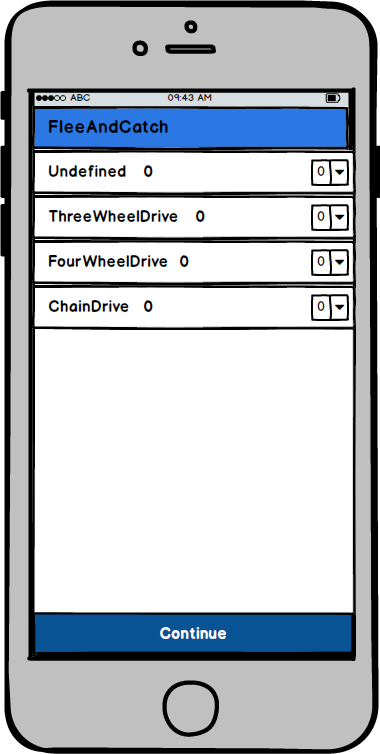
\includegraphics[width=0.5\textwidth]{images/mockups/RobotList.png}
	\end{center}
	\caption{Robot list}
	\label{fig:RobotList}
\end{figure}

\subsubsection{Szenario}

\begin{figure}[h]
	\begin{center}
		\includegraphics[width=0.6\textwidth]{images/use_cases/Spectator.png}
	\end{center}
	\caption{Spectator}
	\label{fig:UC_Spectator}
\end{figure}
\begin{figure}[h]
	\begin{center}
		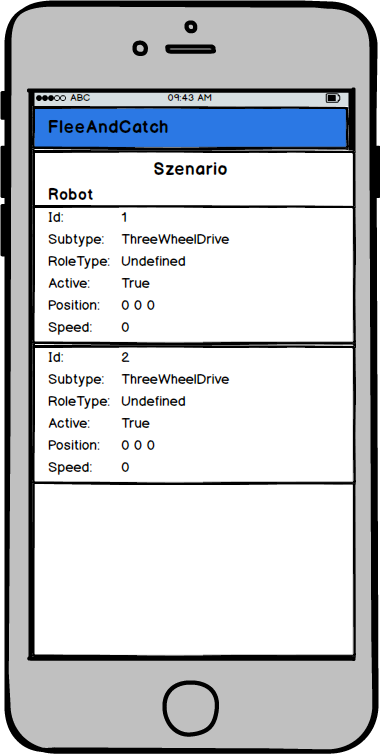
\includegraphics[width=0.6\textwidth]{images/mockups/Spectator.png}
	\end{center}
	\caption{Spectator}
	\label{fig:Spectator}
\end{figure}

\begin{figure}[h]
	\begin{center}
		\includegraphics[width=0.8\textwidth]{images/use_cases/Control.png}
	\end{center}
	\caption{Control}
	\label{fig:UC_Control}
\end{figure}
\begin{figure}[h]
	\begin{center}
		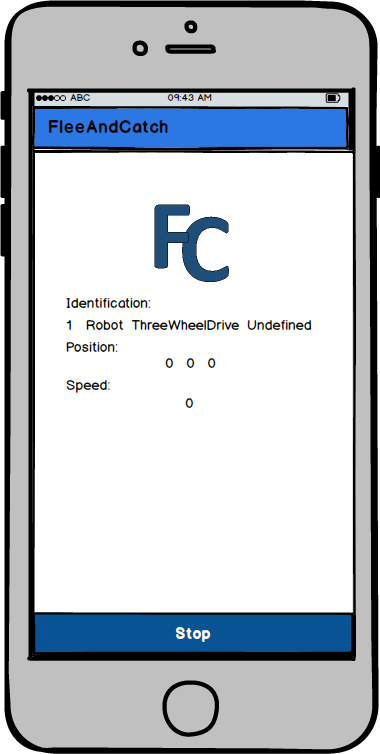
\includegraphics[width=0.6\textwidth]{images/mockups/Control.png}
	\end{center}
	\caption{Control}
	\label{fig:Control}
\end{figure}

\begin{figure}[h]
	\begin{center}
		\includegraphics[width=0.9\textwidth]{images/use_cases/Synchron.png}
	\end{center}
	\caption{Synchron}
	\label{fig:UC_Synchron}
\end{figure}

\begin{figure}[h]
	\begin{center}
		\includegraphics[width=0.9\textwidth]{images/use_cases/Follow.png}
	\end{center}
	\caption{Follow}
	\label{fig:UC_Follow}
\end{figure}

\subsubsection{Exception}
\subsection{Kommunikation}